\documentclass{beamer}

\usepackage{biblatex}
\addbibresource{final.bib}
\usepackage{hyperref}
\usepackage[utf8]{inputenc}

\usepackage{algorithm}
\usepackage{algpseudocode}
\makeatletter
\algrenewcommand\ALG@beginalgorithmic{\footnotesize}
\makeatother

\usetheme{Pittsburgh}
\usecolortheme{default}
\setbeamertemplate{items}[triangle]
\setbeamertemplate{sections/subsections in toc}[square]

%Information to be included in the title page:
\title{Bayesian parameter synthesis for markov population model.}
\author{Nhat-Huy Phung}
\institute{University of Konstanz}
\titlegraphic{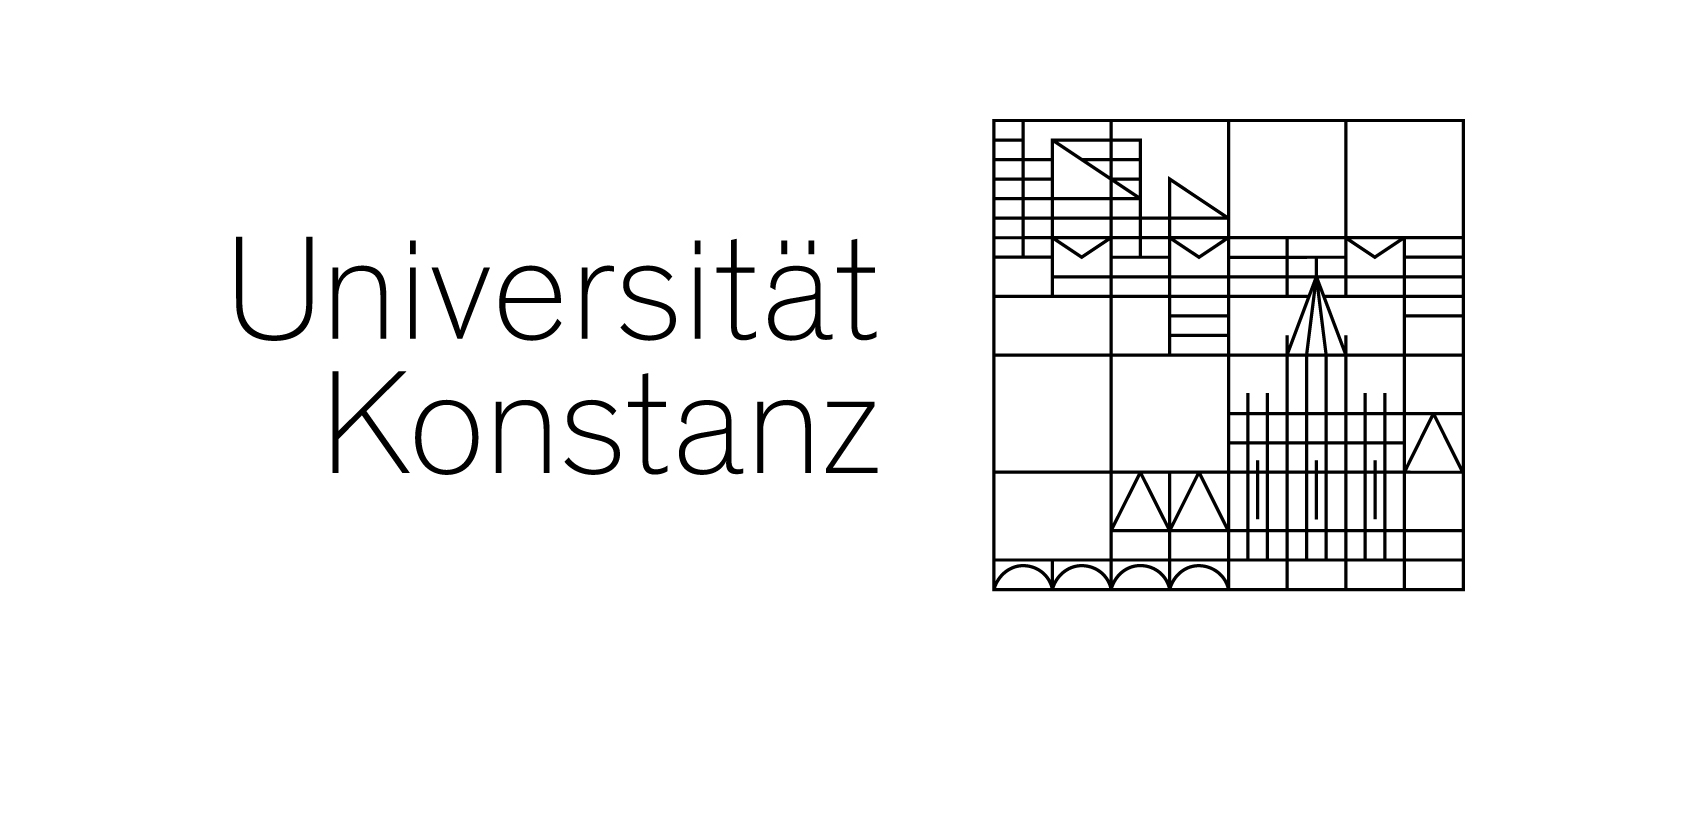
\includegraphics[width=5cm]{figures/unisignet-klein.jpg}}


\begin{document}

\frame{\titlepage}
\frame{\tableofcontents}

\section{Introduction}
\begin{frame}
    \begin{center}
        \Huge Introduction.
    \end{center}
\end{frame}
%% 2 frames

\section{Preliminaries}
\begin{frame}
    \begin{center}
        \Huge Preliminaries
    \end{center}
\end{frame}


%% 5 frames
%% DTMC
%% PCTL
%% pDTMC and parameter synthesis problem
\begin{frame}
    \frametitle{Parameter synthesis}
    Katoen \cite{katoen2016probabilistic} definition
    \begin{definition}[Discrete-time Markov Chain]

    \end{definition}
\end{frame}

\begin{frame}
    \frametitle{Parameter synthesis}
    Katoen \cite{katoen2016probabilistic} definition
    \begin{definition}[PCTL]

    \end{definition}
\end{frame}

\begin{frame}
    \frametitle{Model checking PCTL}
    Katoen \cite{katoen2016probabilistic} definition
    \begin{definition}[PCTL]

    \end{definition}
\end{frame}

\begin{frame}
    \frametitle{Model checking PCTL}
    Katoen \cite{katoen2016probabilistic} definition
    \begin{definition}[PCTL]

    \end{definition}
\end{frame}

\begin{frame}
    \frametitle{Parameter synthesis}
    Katoen \cite{katoen2016probabilistic} definition
    \begin{definition}[Parametric Discrete-time Markov Chain]

    \end{definition}
\end{frame}

\begin{frame}
    \frametitle{Parameter synthesis}
    Katoen \cite{katoen2016probabilistic} definition
    \begin{definition}[Parameter synthesis]
        Given a finite-state parametric Markov model, find the parameter values for which a given
        reachability property exceeds (or is below) a given threshold $\beta$.
    \end{definition}
\end{frame}

\begin{frame}
    \frametitle{Parameter synthesis and Parameter inference}
    What are the differences between parameter inference and parameter synthesis?
    \begin{table}[]
        \begin{tabular}{|l|l|l|}
            \hline
                                       & Input                      & Ouput                      \\ \hline
            \begin{tabular}[c]{@{}l@{}}Parameter\\ inference\end{tabular}  & \begin{tabular}[c]{@{}l@{}}Model $\mathcal{M}_\theta$\\ Observed data $D_{obs}$ \end{tabular}  & \begin{tabular}[c]{@{}l@{}}Parameter estimation\\ $\hat{\theta}$\end{tabular}  \\ \hline
            \begin{tabular}[c]{@{}l@{}}Parameter\\ synthesis\end{tabular} & \begin{tabular}[c]{@{}l@{}}Model $\mathcal{M}_\theta$\\ Reachability property $\Phi$ \end{tabular} & \begin{tabular}[c]{@{}l@{}}$(\theta_1,\ldots,\theta_N)$ \\ $\forall \theta_i \in (\theta_1,\ldots,\theta_N): \mathcal{M}_{\theta_i}\models\Phi$\end{tabular} \\ \hline
        \end{tabular}
    \end{table}
    Synthesis: input: model $\mathcal{M}_\theta$ and property $\Phi$, output is the set of satisfying parameters $\theta$
    Inference: input: model $\mathcal{M}_\theta$ and observed data $D_{obs}$, output is the set of parameter estimation $\hat{\theta}$
    This thesis: combines parameter inference and synthesis into data-informed, Bayesian parameter synthesis frameworks.
\end{frame}

%% Bayesian inference: tractability and optimization

\section{Problem description}
\begin{frame}
    \begin{center}
        \Huge Problem description
    \end{center}
\end{frame}
%% 2 frames

\section{Framework}
\begin{frame}
    \begin{center}
        \Huge Frameworks
    \end{center}
\end{frame}
%% 10 frames

\begin{frame}
    \frametitle{Model checking step}
    A property $\Phi$ is
    \begin{itemize}
        \item a bounded reachability property and
        \item specified by PCTL.
    \end{itemize}
    Checking a model $\mathcal{M}_\theta$ against $\Phi$
    \begin{itemize}
        \item Rational fucntion evaluation
        \item Statistical model checking
    \end{itemize}
\end{frame}

\begin{frame}
    \frametitle{Parameter synthesis step}
    Monte-Carlo Markov chain framework, basically modified Metropolis-Hasting algorithm.
    \begin{algorithm}[H]
        \caption{Markov Chain Monte-Carlo with rational functions}
        \label{rf-mcmc-alg}
        \begin{algorithmic}[1]
            \Procedure{MCMC-RF}{}
            \State Init $\theta$ from prior distribution $\pi(\theta)$.
            \State $i \leftarrow 1$
            \While{$i \leq N$}
            \State Draw $\theta_{cand}$ from $Q(\theta|\theta_1,\ldots,\theta_i)$
            \If{$P(D_{obs}|\theta_{cand}) > P(D_{obs}|\theta_i)$}
            \State Accept $\theta_{cand}$ if $\mathcal{M}_{\theta_{cand}} \models \Phi$
            \State $i \leftarrow i + 1$
            \EndIf
            \EndWhile
            \State Return $(\theta_1,\ldots,\theta_N)$
            \EndProcedure
        \end{algorithmic}
    \end{algorithm}
    Pros: easy to implement, efficient with unimodal
\end{frame}

\begin{frame}

\end{frame}

\begin{frame}
    \frametitle{Parameter synthesis step}
    \begin{algorithm}[H]
        \caption{Sequential Monte-Carlo with rational functions}
        \label{rf-smc-alg}
        \begin{algorithmic}[1]
            \Procedure{SMC-RF}{}
            \State Init $\theta_1,\ldots,\theta_N$ from prior distribution $\pi(\theta)$.
            \State Set  $w_i \leftarrow P(D_{obs}|\theta_i), 1\leq i\leq N$
            \For{$t \in (1,\ldots,M)$}
            \State Normalize $w^t_1,\ldots,w^t_N$
            \State Sample with replacement $\theta^t_1,\ldots,\theta^t_N$ from $\theta^{t-1}_1,\ldots,\theta^{t-1}_N$
            \For{$\theta_i \in (\theta^t_1,\ldots,\theta^t_N)$}
            \State $\theta_i \leftarrow MCMC-RF(\theta_i)$, $Q = F_i(\theta|\theta^{t-1}_1,\ldots,\theta^{t-1}_N)$
            \EndFor
            \EndFor
            \State Return $(\theta_1,\ldots,\theta_N)$
            \EndProcedure
        \end{algorithmic}
    \end{algorithm}
\end{frame}

\begin{frame}
    \frametitle{Parameter synthesis step}
    \begin{algorithm}[H]
        \caption{Sequential Monte-Carlo with simulations}
        \label{smc-abc-smc-alg}
        \begin{algorithmic}[1]
            \Procedure{RF-SMC}{}
            \State Init $\theta_1,\ldots,\theta_N$ from prior distribution $\pi(\theta)$.
            \For{$t \in (1,\ldots,M)$}
            \State Sample with replacement $\theta^t_1,\ldots,\theta^t_N$ from $\theta^{t-1}_1,\ldots,\theta^{t-1}_N$
            \For{$\theta_i \in (\theta^t_1,\ldots,\theta^t_N)$}
            \State Draw $\theta_{cand}$ from $F_i(\theta|\theta^{t-1}_1,\ldots,\theta^{t-1}_N)$
            \If{Statistical Model Checking $\mathcal{M}_{\theta_{cand}} \models \Phi$}
            \State Simulate $D_{sim}$ from $\mathcal{M}_{\theta_{cand}}$
            \If{$Distance(D_{sim}, D_{obs} < \epsilon)$}
            \State Update $\theta_i \leftarrow \theta_{cand}$
            \EndIf
            \EndIf
            \EndFor
            \EndFor
            \State Return $(\theta_1,\ldots,\theta_N)$
            \EndProcedure
        \end{algorithmic}
    \end{algorithm}
\end{frame}


\begin{frame}[allowframebreaks]{References}
    \printbibliography
\end{frame}

\end{document}